\documentclass[11pt]{article}

\usepackage{amssymb}
\usepackage[english]{babel}
\usepackage{changepage}
\usepackage{cite}
\usepackage{float}
\usepackage[margin=1.5in]{geometry}
\usepackage{graphicx}
\usepackage{lmodern}
\usepackage{setspace}
\usepackage{tabularx}
\usepackage{booktabs}
\usepackage[table,xcdraw]{xcolor}
\usepackage{adjustbox}
\usepackage{url}
\usepackage{listings}
\usepackage{appendix}

\usepackage[T1]{fontenc}

\bibliographystyle{ieeetr}

\graphicspath{{figures}}

\lstset{
    basicstyle=\small,
    showspaces=false,
    showstringspaces=false,
    tabsize=2,
    title=\lstname,
}

\onehalfspacing

\begin{document}
\thispagestyle{empty}
\begin{center}
\begin{Large}
\emph{Thesis Submitted for Master of Science in Computer Science} \\
Department of Computer Science \\
Rochester Institute of Technology \\
\end{Large}
\vspace{4em}
{\huge Generalized Model of Cognitive Workload} \\
\vspace{3em}
{\LARGE Taylor Carpenter} \\
{\tt tjc1575@rit.edu} \\
\vspace{3em}
\begin{adjustwidth}{.5in}{.5in}
Chair: Dr. Zack Butler \hfill {\tt zjb@cs.rit.edu} \\
\vspace{2em}
\hrulefill \\
\vspace{3em}
Reader: Dr. Esa Rantanen \hfill {\tt emrgsh@rit.edu} \\
\vspace{2em}
\hrulefill \\
\vspace{3em}
Observer: Sean Strout \hfill {\tt sps@cs.rit.edu} \\
\vspace{2em}
\hrulefill
\end{adjustwidth}
\vspace{2em}
Rochester, NY 14623 USA \\
\vspace{2em}
\today
\end{center}
\pagebreak
\thispagestyle{empty}
\begin{center}
\begin{large}
A Thesis Submitted\\
in\\
Partial Fulfillment of the\\
Requirements for the Degree of\\
Master of Science in Computer Science

\vspace{.5in}

Department of Computer Science\\
B. Thomas Golisano of Computing and Information Sciences\\
Rochester Institute of Technology\\
Rochester, NY 14623 USA
\end{large}
\end{center}
\pagebreak
\thispagestyle{empty}
\begin{abstract}
\noindent
\end{abstract}
\clearpage
\pagenumbering{arabic}
\tableofcontents
\listoffigures
\listoftables
\pagebreak

\section{Introduction}
% General introduction stuff
% What is the research area?
a
	
d		

\section{Background}
e
	\subsection{Terminology}
	% Cognitive Workload
	% "Study"
	% "System"
	% "Model"
f	
	\subsection{Cognitive Workload}
	% What is it?
	% Current / previous research into workload
g	
	\subsection{Physiological Measures}
	% What measures have been used in this line of research?
		% EEG
		% HR
		% Eye movement
		% Respiration
		% Cranial blood flow
	% When did EEG start being used as a measure of workload?
	% What does EEG show?
h	
	\subsection{Random Forest}
	% What is it?
	% Who first created it?
	% Why are ensemble methods useful?
	% What can be tuned?
	% Pros / Cons
i	
	\subsection{Artificial Neural Network}
	% What is it?
	% Who first created it?
	% What can be tuned?
	% Pros / Cons
j
\section{Related Work}
% All the references and everything of existing work like this
k
\section{Problem Statement}
% How is this research different than existing research
% What is the hypothesis that we are trying to solve?
	\subsection{Applications}
	% Why is this research important?
b	
		\subsubsection{Adaptive Automation}
		% What is adaptive automation?
		% How does a workload classifier interact with AA?
		% Maintain ideal level of interaction between system and human
		% Why is high workload bad?
		% Why is low workload bad?
		% Existing research related to adaptive automation 
c		
		\subsubsection{Research}
		% Some tasks are easier to control workload than others
		% Can increase understanding of difficult to control tasks
l
\section{Study}
A study was conducted in order to generate and collect the data needed to train the appropriate models. While some previous research~\cite{cross research I believe} has relied on the use of established and validated data collected from other experiments~\cite{main Wilson paper}, the amount of data required to adequately train artificial neural networks was not available. Consequently, a new study was required to generate the large amount of data that was necessary. The study consisted of two tasks, each with three load conditions and a leading baseline trial. The load condition trials were ten minutes long and the baseline trials were five minutes long. 
{\bf The initial design of the study specified fifteen minute long trials but feedback from the pilot group suggested that at fifteen minutes, task fatigue started affecting performance. } % Is this necessary and is it obvious that the feedback resulted in the change to 10 minutes?

%% Transition?

The study began with a total of ten college-aged participants, similar to existing works~\cite{ ... }, however, due to complications, only seven participants completed the entire process. 
{\bf Two of the removed participants were excluded due to misfitting of the EEG headset as well as discrepancies between the task difficulties reported versus the average difficulties reported by the other participants. The last removed participant was excluded due to personal issues preventing the completion of the study.} % Check this sentence...
Of the seven participants that completed the study, the ages ranged from 18 to 23 years old, with an average age of 21.1 years old. The gender ratio was balanced with three males and four females. Participants lacked any uncorrected hearing or visual impairments that would affect performance on the tasks of the study. 
{\bf The following subsections describe each of the tasks as well as the overall layout of the study in its entirety. } % Is this a weird transition?
	
	\subsection{Multi-Attribute Task Battery ( MATB )}
	The first task presented to participants is the Multi-Attribute Task Battery (MATB), a task loading system originally developed by NASA ~\cite{}. MATB is a system that has been used in a variety of studies as a means of task loading for the collection of psychophysiological data~\cite{...}. The system consists of a multitude of subtasks arranged in such a way as to simulate the tasks a pilot might be required to perform during flight. The particular version of the system used in this study is AF-MATB, an updated version of the original software~\cite{...}. This version is very similar to the original with the majority of the changes affecting how it runs on modern operating systems and adding different options for subtask automation. All of the subtasks of MATB were used in the study, while the scheduling view that shows upcoming events was disabled. This included resource management, systems monitoring, communications, and tracking. Input to the system was in the form of joystick for the tracking subtask and either keyboard or mouse for the remaining tasks. Participants were free to decide whether to use the keyboard, mouse, or a combination of the two with the right hand while the joystick was controlled with the left hand. In Figure~\ref{fig:matb}, the main view of MATB with which participants interacted is shown. 
	
	\begin{figure}[]
	\centering
	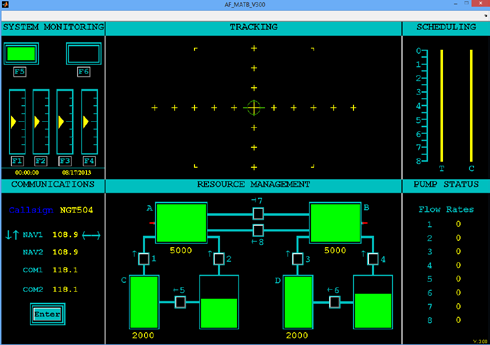
\includegraphics[width=\linewidth]{figures/matb.png}
	\caption{Main view of the MATB simulation software. }
	\label{fig:matb}
	\end{figure}
	
	The resource management subtask involved maintaining the amount of fuel that was present in two main tanks within a small acceptable range. Secondary tanks were present and could be used to temporarily store fuel. The participant was required to toggle pumps, controlling the flow of fuel between the tanks. Throughout the trial, pumps would temporarily break, or silently shut-off, preventing the flow of fuel through the pump. The number and frequency of these occurrences depended on the difficulty condition.
	
	The systems monitoring subtasks were centered around two buttons and four gauges. One button was to be kept on while the other button was to be kept off. Throughout the simulation, the buttons changed states and the participant was required to click on the button indicator, or press a corresponding key, to revert the button to the correct state. Colors were used to indicate the state of the buttons. Background color indicated that the button was off, while either red, for the ``off'' button, or green, for the ``on'' button, was used to indicate on. The gauges presented had sliders that would vary in vertical position throughout the simulation. Occasionally, depending on the difficulty condition, a slider would move outside the acceptable range for the gauge and require interaction from the participant, either through a mouse click or key press, to reset the gauge. If an out-of-state system component was not addressed within the response time period of ten seconds, the component was automatically reset to its defaults, within-range state.
	
	The communication subtask required the use of sound. For the duration of the simulation, the participant was assigned a {\bf particular aircraft callsign for which they were required to listen. } The communication window included four different communication channels, each set to a particular frequency. Throughout the simulation, recorded audio tracks would play, addressing a particular callsign to change a channel to a desired frequency. If the callsign matched that of the participant, they were to change the specified communication channel to the appropriate frequency using either the mouse of the arrow keys. If the callsign did not match that of the participant, the request was to be ignored. The number and rate of true- and false-alarm requests depended on the difficulty condition of the trial.
	
	The tracking subtask was the only subtask that required the use of the joystick. In this subtasks, the participant simulated steering a plane by keeping a reticle within the acceptable parameters of the tracking window. The amount of drift affecting the reticle and the amount of control the joystick emitted onto the reticle varied throughout the simulation in accordance with the difficulty condition. 
	
	\begin{table}[]
	\centering
	\adjustbox{max width=\textwidth}{
	\begin{tabular}{llllllll}
	\toprule
	\rowcolor[HTML]{FFFFFF} 
	 &  & \multicolumn{2}{c}{\cellcolor[HTML]{FFFFFF}Communication} & \multicolumn{2}{c}{\cellcolor[HTML]{FFFFFF}System} & \multicolumn{2}{c}{\cellcolor[HTML]{FFFFFF}Resources} \\ \cmidrule(l){3-8} 
	\rowcolor[HTML]{FFFFFF} 
	Load Condition & Tracking & Target & Distractor & Lights & Gauges & Failures & Shut-offs \\ \midrule
	\rowcolor[HTML]{EFEFEF} 
	Low & Low & 6 & 2 & 48 & 42 & 4 & 2 \\
	\rowcolor[HTML]{FFFFFF} 
	Moderate & Moderate & 18 & 10 & 96 & 102 & 20 & 10 \\
	\rowcolor[HTML]{EFEFEF} 
	High & High & 30 & 12 & 110 & 120 & 40 & 20 \\ \bottomrule
	\end{tabular}
	}
	\caption{Parameter values for MATB task for each load condition.}
	\label{tab:matb-params}
	\end{table}
	
	The baseline condition for MATB involved the participant watching the screen while the simulation ran with the low condition parameters and automation of all available tasks enabled. {\bf This allowed for the visual stimulation that was present in performing the task without the cognitive workload. } Presented in Table~\ref{tab:matb-params} are the parameter values that were entered into the script generator of MATB to produce the trials for each load condition. Two scripts were generated for each difficulty condition to ensure that each trial was different and the participants could not memorize any patterns. The parameter values used are based off those in a previous study ~\cite{...}. The majority of the parameter values are scaled from the referenced values to account for the difference in trial lengths, however the parameters for ``lights'' and ``gauges'' in the high condition were further modified due to errors in scheduling from the script generator. 
	
	
	\subsection{RanTask}
	The second loading task used in this study is a custom tone counting task, referred to herein as RanTask. This task is an extension of the mental workload loading task used in the work of Rantanen et al.~\cite{Rantanen}. The participant was presented with three different tones in a random order. The task of the participant was to count the tones that were presented and press the key corresponding to the tone when the desired count was reached. The intended count differed with the difficulty condition. The tones corresponded to the notes B at 493 Hz, F at 698 Hz, and A at 880 Hz. Each tone was presented for one second with a one second interval between tones, giving the participant two seconds to respond to a given tone. Each time a tone was presented, a log entry was created, recording the tone presented, its number in the sequence, and whether, if a participant pressed a key, it was correct or incorrect. If a key was pressed at an incorrect time, a false-positive was logged and the sequence count for the corresponding tone was reset to prevent cascading failure, e.g. counting every five correctly but being off by one from the ground truth sequence would result in all false-positive without the reset. 
	
	\begin{table}[]
	\centering
	\adjustbox{max width=\textwidth}{
	\begin{tabular}{llll}
	\toprule
	\rowcolor[HTML]{FFFFFF} 
	 & \multicolumn{3}{c}{\cellcolor[HTML]{FFFFFF}Tone Frequency} \\ \cmidrule(l){2-4} 
	\rowcolor[HTML]{FFFFFF} 
	Load Condition & Low & Moderate & High \\ \midrule
	\rowcolor[HTML]{EFEFEF} 
	Low & 0 & 5 & 0 \\
	\rowcolor[HTML]{FFFFFF} 
	Moderate & 2 & 0 & 3 \\
	\rowcolor[HTML]{EFEFEF} 
	High & 2 & 2 & 3 \\ \bottomrule
	\end{tabular}
	}
	\caption{Desired counts for each tone in each load condition.}
	\label{tab:rantask-params}
	\end{table}
	
	In the baseline trial, the participant was not required to count any of the tones, only listen. Presented in Table~\ref{tab:rantask-params} are the desired counts for each tone in each load condition. This differ from the originally intended counts due to feedback from the pilot study members. Feedback indicated that the original low- and moderate-load conditions, both requiring the counting of a single tone, were too similar in difficulty. As such, the moderate-load condition was replaced and an additional condition was added that required keeping count of all three tones. {\bf The participants were presented with the count information at the time of the trial to ensure the participants were aware of which tones were to be counted. The participants were also informed that the use of fingers for counting or any other external methods of keeping track of tones was prohibited. }

	% Talk about the fact that a demo of the tones was presented before each trial?
	
	\subsection{NASA Task Load Index (TLX)}
	The NASA Task Load Index (TLX) survey is a means of determining the workload for a given task based on participant responses~\cite{}. The procedure allows for exploring the different aspects of a task and where the underlying cognitive workload originates. The workload rating obtained from participants through the TLX process was used to compare the subjective difficulties of the various tasks, similar to the procedure used in existing studies~\cite{}. The current TLX procedure consists of six subscales: Mental Demands, Physical Demands, Temporal Demands, Own Performance, Effort, and Frustration. The mental subscale measures how much mental activity was required and its complexity. Physical Demands measures how much physical activity was required and how laborious it was. Temporal Demands measures how much time pressure was present in the task. In the performance subscale, the participant remarks on how successful they felt they were and how satisfied they are with their performance. The effort subscale measures how hard the participant had to work to accomplish the task. The final subscale, frustration level, measures how stress or relaxed the participant felt during the task. 
	% Check tenses, do they make sense?
	
	Individual calibration was required from each participant for both of the tasks that were performed. During this calibration, the participant performs pair-wise comparisons between the TLX subscales, indicating which subscales had more effect on the overall workload of the task. The calibration is then used as a method of weighting the individual TLX survey responses for a trial. The idea behind the weighting is that a component that is calibrated as having a large impact on the overall workload should have its rating affect the overall workload more heavily. In addition to the weighting of individual trial ratings, the calibration also allows for comparisons between tasks in how they affect participants.
	% Is the point of this clear?
		
	\subsection{Structure} % Setup?
	The study took place over four days for each participant. Each day required roughly an hour and a half from the participant. The time is approximate as it was dependent on how quickly the sensors were placed, which was, at times, delayed due to conditions such as hair. The first day consisted of an introduction to the system: what sensors were to be utilized, the intent of the study, and what was to be expected of the participant. Training was also conducted on each task to familiarize the participant with what was to be expected. Ideally, stable performance on both tasks was achieved for all participants as a result of training. Other studies~\cite{Wilson} have included lengthier training periods, however, due to time constraints, the time required for complete stability was not feasible. 
	{\bf As such, the performance results of each participant was recorded and examined and will be discussed later in this paper as a factor in the overall effectiveness of this study. } % Does this sound okay, referencing itself?
	
	The second day marked the beginning of data collection for the participants. The participants were attached to the sensors and a five minute baseline recording using MATB was taken. Following the baseline, the participants each completed a ten minute MATB trial on the low-load condition. A NASA TLX survey was then administered to record the participants' rating of the task workload. Next, the participants completed a second, ten minute MATB trial on the low-load condition. This again was followed by a NASA TLX survey. Two TLX surveys were taken for each condition to evaluate the stability of the rating as participants should be recording similar ratings for both trials of a condition. After a ten minute break, the same procedure was repeated, including the baseline, substituting RanTask for MATB as the task being performed.
	
	The third and fourth days followed the same format as the second day. The third day consisted of the tasks being performed on the moderate-load condition while the fourth day consisted of the tasks being performed on the high-load condition. The order in which the load conditions were presented follows that of a previous study~\cite{Wilson}. {\bf While the sensors were removed and replaced on multiple occasions as the data collection occurred over many days, which differs from some studies~\cite{Wilson, ...}, this should not have an effect on the overall validity of the data~\cite{...}}


\section{System}
% Overview of the whole system, what parts are involved
% Diagram showing the how the different parts interact
r
	\subsection{Sensors}
	% How was data collected?
	% When was data collected?
		% Noise on either end requiring processing
s		
		\subsubsection{Electroencephalogram (EEG)}
		% How was EEG recorded?
			% Headset specs
		% Headset was cheaper than alternatives
		% Headset required less expertise on placement
t			
		\subsubsection{Heart Rate}
		% How was heart rate recorded?
			% Heart rate monitor specs
		% Arm based was used as it is less intrusive
u		
	\subsection{Data Preprocessing}
	% Overview of what preprocessing had to be done
v	
		\subsubsection{EEG}
		% Diagram of EEG preprocessing
		% How was EEG preprocessed?
			% EEG edf to plain text file
				% Baseline / mean signal removed
			% total file times expanded from offset to full time
			% total file split into individual channel files
			% partition each file into 5-second intervals
w			
		\subsubsection{Heart Rate}
		% Diagram of HR preprocessing
		% How was heart rate preprocessed?
			% Smoothing / interpolation
			% Partition data into 5-second intervals
x			
	\subsection{Data Processing and Features}
	% Overview of what processing had to be done
	% Condition information gets labeled and added to one record
y	
		\subsubsection{EEG}
		% Diagram of EEG processing
		% How was EEG processed?
			% FFT on each 5-second interval
			% Logs of band sections taken and summed
z			
		\subsubsection{Heart Rate}
		% Diagram of HR processing
		% How was HR processed?
			% Removed baseline from each entry
			% compute average HR and HRV
a			
	\subsection{Classifiers}
	% What classifiers are being created?
	% talk about both RF and ANN
	% Talk about training times
	% Talk about libraries
	% What parameters are being held constant?
	% What parameters are being tuned?
b
		\subsubsection{Random Forest}
		\subsubsection{Artificial Neural Network}
		
	\subsection{Configurations}
	% Each configuration talks about what it is supposed to cover, what configuration of train / test
		\subsubsection{Same Participant - Same Task (SP-ST)}
		\subsubsection{All Participants - Same Task (AP-ST)}
		\subsubsection{Same Participant - All Tasks (SP-AT)}
		\subsubsection{All Participants - All Tasks (AP-AT)}
		\subsubsection{Cross Participant - Same Task (CP-ST)}
		\subsubsection{Same Participant - Cross Task (SP-CT)}
		\subsubsection{All Participant - Cross Task (AP-CT)}
		\subsubsection{Cross Participant - All Tasks (CP-AT)}
		\subsubsection{Cross Participant - Cross Task (CP-CT)}
c
\section{Results}
% What is the layout of this section?
d
	\subsection{Study}
	% Why do the performance and TLX results matter?
		% Show how well the tasks induced the right behavior
e		
		\subsubsection{Performance}
		% Tables and graphs of performance data
		% Average performances etc.
f		
		\subsubsection{NASA Task Load Index ( TLX )}
		% Tables and graphs of TLX data
		% Average ratings etc.
g		
	\subsection{Classifier Models}
	% Results of each of the configurations
	% For configurations with multiple models, report average
	% ** FOCUS IS NOT ON WHICH MODEL METHOD IS BETTER **
h	
		\subsubsection{Same Participant - Same Task (SP-ST)}
		% Box graph of MATB and RanTask, one for ANN and one for RF
		
		\subsubsection{All Participants - Same Task (AP-ST)}
		% Bar graph of MATB and RanTask, one for ANN and one for RF
		
		\subsubsection{Same Participant - All Tasks (SP-AT)}
		% Box graph of both, one for ANN and one for RF
		
		\subsubsection{All Participants - All Tasks (AP-AT)}
		
		\subsubsection{Cross Participant - Same Task (CP-ST)}
		% Box graph of MATB and RanTask, one for ANN and one for RF
		
		\subsubsection{Same Participant - Cross Task (SP-CT)}
		% Box graph of both.
		
		\subsubsection{All Participant - Cross Task (AP-CT)}
		% Bar graph of MATB and RanTask, one for ANN and one for RF
		
		\subsubsection{Cross Participant - All Tasks (CP-AT)}
		%Box graph, one for ANN and one for RF
		
		\subsubsection{Cross Participant - Cross Task (CP-CT)}
i
		
\section{Discussion}
% What is discussion going to cover?
j
	\subsection{Study}
	% How effective was the study is doing what it was supposed to?
	% Do the trends in the results look like expected?
	% Plot of Performance vs TLX
k	
	\subsection{Classifier Models}
	% How do the individual models look?
		% Compare to existing study results
	% Did it generalize well?
	% What may have been the issue in generalizing?
		% People are different ( HR is accounted for but not EEG, research that shows EEG is different in people )
		% Tasks may have been too different
	% Why are there discrepencies in the accuracies of ANN and RF
l	
	\subsection{Potential Sources of Error}
	% Each difficulty was on its own day
		% Possible reasons why that is not an issue
	% Different people may have thought the tasks were of different difficulties
	% Headset is sensitive to noise
	% More tuning
m
\section{Future Work}
% More similar tasks
% More people
% Different modeling methods
	
\section{Conclusion}
% Was it successful / hypothesis proven?
% Other comments on the overall outcome
p	

\pagebreak
\bibliography{references}

\pagebreak
\begin{appendices}
\appendixpage
\noappendicestocpagenum
\addappheadtotoc
\section{NASA Task Load Index Records}
\section{Performance Data}
	\subsection{Multi-Attribute Task Battery}
	\subsection{RanTask}
\section{Model Performance}
\section{Study Source Code}
	\subsection{Performance Metrics}
\section{System Source Code}
	\subsection{Data Preprocessing}
	\subsection{Data Processing / Feature Generation}
	\subsection{Model Training}
\end{appendices}	
\end{document}




















